\section{Aufgabe 3}
In dieser Aufgabe wurde eine Wechselstrombrücke aufgebaut um sowohl die Induktivität \(L_x\) als auch den Ohmschen Widerstand \(R_x\) der Spule vom Tiefpass aus Aufgabe 2 zu bestimmen. 

\subsection{Aufbau}
Hierfür wurde eine Schaltung auf dem Steckbrett nach folgendem Schaltplan aufgebaut. Die Phase zwischen den beiden Spannungsmesspunkten wurde mit dem Oszilloskop mit der ,,elliptischen Auftragung'' auf \(\varphi = 0 \) eigestellt. Und anschließend die Effektivspannung mit dem Fluke 175 gemessen
\begin{center}
\begin{minipage}{\linewidth}
\centering
\makebox[0cm]{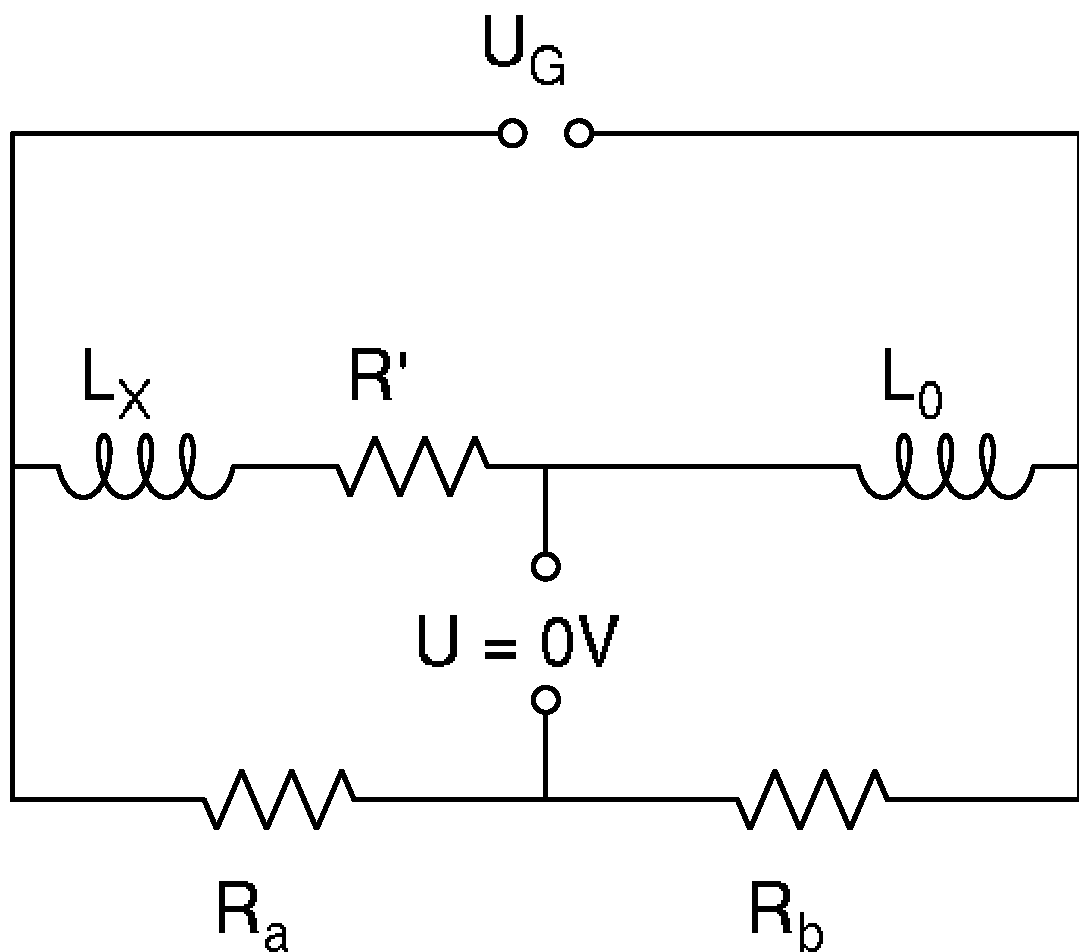
\includegraphics[width=6cm]{bilder/bruecke}}
\captionof{figure}{Schaltplan der Wechselstrombrücke}
\end{minipage}
\end{center}

\subsection{Gegebenes und Messwerte}
Separat wurden folgende Größen gemessen oder von den Aufschriften der Bauteile entnommen. Leider wurde vergessen zu notieren mit welchem Messgerät die Widerstände gemessen wurden die Fehler werden mit \(\Delta R = 1\% + 5d\) abgeschätzt.
\begin{center}
\begin{tabular}{c|c}
Messgröße & Messwert\\\hline
\(f\) & \((1999 \pm 14)\, Hz \) \\
\(L_0\) & \((1,507 \pm 0,020)\, mH \) \\
\(R_0\) & \((2,91 \pm 0,02)\, \Omega \) \\
\(R_a\) & \((761 \pm 13)\, \Omega \) \\
\(R_b\) & \((241,8 \pm 2,9)\, \Omega \) \\
\(R'\) & \((5,3 \pm 0,5)\, \Omega \) \\
\(f\) & \((1999 \pm 14)\, Hz \) \\ \hline
\(R_x\) & \(\left(3,7 \pm 0,5 \right)\, \Omega \) \\
\(L_x\) & \((4,82\pm 0,07)\, mH \) \\
\end{tabular}
\captionof{table}{Sepperate Messung aller Größen}%
\end{center}

\subsection{Auswertung}
Um nun aus den Vorhanden Messdaten \(L_x\) und \(R_x\) zu bestimmen, wird folgender Ansatz gemacht:
\begin{align}
\frac{Z_a}{Z_b} &= \frac{i\omega L_x + R'+ R_x}{i\omega L_0 + R_0}
\end{align}
Da über den Phasenabgleichswiderstand die Phase auf \(\varphi = 0\) gebracht wurde müssen die beiden Phasenverschiebungen der Spulen und Widerständen identisch sein. Daher gilt:
\begin{align}
\Rightarrow \frac{i\omega L_0}{R_0} &= \frac{i\omega L_x}{R'+R_x}\notag \\
\Rightarrow L_x &= \frac{L_0}{R_0}\cdot\left( R' + R_x \right) \label{L_x}
\end{align}
Außerdem wurden \(R_a\) und \(R_b\) derart gewählt, dass gelten muss:
\begin{align}
\frac{R_a}{R_b} &= \frac{\omega L_x + R' + R_x}{\omega L_0 + R_0}
\end{align}
Nach einsetzten von \eqref{L_x} formt sich das zu
\begin{equation}
R_x = \frac{R_a}{R_b} \cdot R_0 - R'
\end{equation} um.
Für die Fehler gilt nach Gaußscher Fehlerfortpflanzung:
\begin{align}
\Delta R_x &= \sqrt{
\left( \frac{R_0}{R_b} \cdot \Delta R_a \right)^2 +
\left( \frac{R_a}{R_b} \cdot \Delta R_0 \right)^2 +
\left( \frac{R_a}{R_b^2} \cdot \Delta R_b \right)^2 +
\left( \Delta R' \right)^2
}\notag \\
\Delta L_x &= \sqrt{
\left( \frac{R'+R_x}{R_0} \Delta L_0 \right)^2 +
\left( \frac{L_0\left( R'+R_x \right)}{R_0^2}  \cdot \Delta R_0 \right)^2 +
\left( \frac{L_0}{R_0} \cdot \Delta R' \right)^2 +
\left( \frac{L_0}{R_0} \cdot \Delta R_x \right)^2
}\notag
\end{align}
Ausgerechnet ergibt das:
\begin{center}
\begin{tabular}{c|c}
Messgröße & Errechneter Wert\\\hline
\(R_x\) & \(\left(3,86 \pm 0,23 \right)\, \Omega \) \\
\(L_x\) & \((4,74\pm 0,50)\, mH \) \\
\end{tabular}
\captionof{table}{Mit der Apparatur ermittelte Größen}
\end{center}

\subsection{Fazit}
Die ermittelten werte für die Induktivität und den ohmschen Widerstand der Spule sind identisch zu den direkt mit dem Messgerät gemessenen Werten. dabei konnte sogar die Genauigkeit der Widerstandsmessung der Spule erhöht werden, da diese sonst nur mit dem für kleine Widerstände sehr ungenauem VC230 oder Fluke 175 gemessen werden konnten.
\begin{center}
\begin{tabular}{c|c|c}
Messgröße & Errechneter Wert & Vergleichswert\\\hline
\(R_x\) & \(\left(3,9 \pm 0,3 \right)\, \Omega \) &  \(\left(3,7 \pm 0,5 \right)\, \Omega \)\\
\(L_x\) & \((4,7\pm 1,7)\, mH \) & \((4,82\pm 0,07)\, mH\) \\
\end{tabular}
\captionof{table}{Mit der Apparatur ermittelte Größen}
\end{center}

\section{Fazit}
Alle drei Aufgaben waren sehr gut durchführbar. Alle Geräte haben durchgehend funktioniert und waren leicht zu bedienen. Besonders das moderne Oszilloskop sorgte für vergleichsweise gute Messdaten. Die Ergebnisse waren zufriedenstellend und wir können die Versuche zu den Wechselstromkreisen auf jeden Fall zu den angenehmen und gleichzeitig interessanten Versuchen zählen.